\documentclass[aspectratio=169]{beamer}
\usepackage{graphicx}
\usepackage{amsmath}
\usepackage{amsthm}
\usepackage{amssymb}
\usepackage{natbib}
\usepackage[T1]{fontenc}
\usepackage[utf8]{inputenc}
\usepackage[english]{babel}
\usepackage{bm}
\usepackage{hyperref}
\usepackage{xcolor}
\usepackage{booktabs}
\usepackage{soul}
\usepackage{algorithm2e}

\newcommand{\bruno}[1]{\textcolor{blue}{#1}} % Bruno Sanso edits- blue
\newcommand{\findcite}{{\color{red} [Find Citation]}}
\newcommand{\needcite}{\findcite}
\newcommand{\makenote}[1]{{\color{red} #1}}
\newcommand{\Chi}{\mbox{\Large$\chi$}}
\newcommand{\norm}[1]{\left\lVert #1 \right\rVert}
\newcommand{\inorm}[1]{\norm{#1}_{\infty}}
\newcommand{\pnorm}[2]{\norm{#1}_{#2}}

\newtheorem{prop}{Proposition}

\DeclareMathOperator{\tr}{Tr}
\DeclareMathOperator*{\argmin}{arg\,min}
\DeclareMathOperator*{\argmax}{arg\,max}

\usetheme{Berlin}
\setbeamertemplate{navigation symbols}{}
\setbeamertemplate{mini frames}{}
\setbeamertemplate{footline}{}
\renewcommand*{\slideentry}[6]{}

\bibliographystyle{plainnat}

\makeatletter
\newlength{\frameheadheight}
\setlength{\frameheadheight}{2cm}
\newlength{\frametextheight}
\setlength{\frametextheight}{\paperheight}
\addtolength{\frametextheight}{-\footheight}
\addtolength{\frametextheight}{-\headheight}
\addtolength{\frametextheight}{-\frameheadheight}
\makeatother

\setcounter{tocdepth}{1}

\title{Multivariate Extreme Value Theory \\ and Applications to Anomaly Detection}
\author{Peter Trubey \\ Advisor: Bruno Sans{\'o}}
\institute{UCSC - Statistics Department}
\date[8/25/2021]{August 25, 2021}

\begin{document}

\begin{frame}[plain]
  \titlepage
\end{frame}

\begin{frame}[plain]
  \frametitle{Overview}
  \tableofcontents
\end{frame}


\section{Introduction}
\subsection{Motivating Example}
\begin{frame}
  \frametitle{Integrated Vapor Transport}
  \begin{minipage}{.7\textwidth}
    \begin{itemize}
        \item Atmospheric rivers~\citep{ralph2013,ralph2018}
            \begin{itemize}
                \item Concentrated water vapor in atmosphere
                \item Huge amounts of water
                \item Predominant source of precipitation for inland California
                \item Extreme behavior has large implications for land use, agriculture, flood prevention/mitigation
            \end{itemize}
        \item The data~\citep{guan2015}
            \begin{itemize}
                \item 42 years of daily average of total water content in atmospheric column above grid cell
                \item Grid cells cover coast of California in two spatial resolutions (8, and 47 cells)
                \item subset to rainy season (November to March)
            \end{itemize}
    \end{itemize}
  \end{minipage}
  ~\hfill
  \begin{minipage}{.25\textwidth}
    \centering
    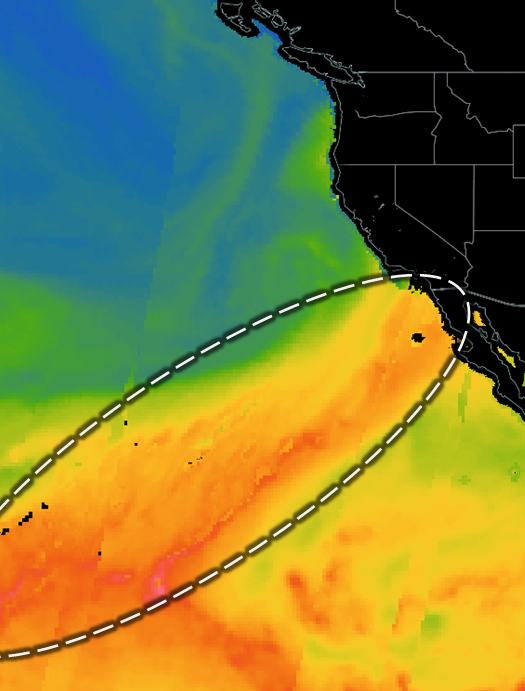
\includegraphics[width=\textwidth]{./images/ar}\\
    {\scriptsize Credit: NASA}
   \end{minipage}
\end{frame}

\subsection{Extreme Value Theory}

\begin{frame}
  \frametitle{Extreme Value Theory - A Brief Background}
  \begin{itemize}
    \item Why EVT?
        \begin{itemize}
            \item Inference on the tails of the distribution
            \item Inference beyond observed sample
            \item Return levels (100 year flood, etc.)
        \end{itemize}
    \item Block Maxima
        \begin{itemize}
            \item \citet{frechet1927,fisher1928,gumbel1942,jenkinson1955}
        \end{itemize}
    \item Threshold Exceedances
        \begin{itemize}
            \item \citet{pickands1975,balkema1974}
        \end{itemize}
    \item Multivariate EVT - more difficult
  \end{itemize}
\end{frame} % EVT Background
\begin{frame}
    \frametitle{Notation}
    \begin{itemize}
      \item Wedge Operators
        \begin{equation*}
            a \vee b = \max(a,b) \hspace{1cm} a\wedge b = \min(a,b)
        \end{equation*}
      \item Positive orthant of unit $d$-sphere under $\mathcal{L}_{\infty}$ norm
        \begin{equation*}
          \mathcal{S}_{\infty}^{d-1} = \left\lbrace \bm{s} : \bm{s} \in [0,1]^d,\hspace{0.2cm}
                            \vee_{l=1}^d s_l = 1\right\rbrace
        \end{equation*}
    \end{itemize}
    
\end{frame} % Notation

\subsection{EVT - Block Maxima}

\begin{frame}
  \frametitle{Block Maxima - Fisher-Tippett-Gnedenko Theorem}
  {\scriptsize\cite{dehaan2006}}\\~\vspace{0.01cm}\\
  For $x_i \stackrel{\text{iid}}{\sim} F$, Let $M_n = \vee_{i=1}^n x_i$.
  \begin{itemize}
    \item If there exists a sequence of constants $a_n > 0$, $b_n$ such that:
        \begin{equation*}
            \text{Pr}\left[\frac{M_n - b_n}{a_n} \leq z\right] \xrightarrow[\enskip n\to\infty\enskip]{} G(z),
        \end{equation*}
        Then $G$ is a \emph{max-stable distribution}, and $F$ is in its \emph{domain of attraction}
    \item 3 possible forms~\citep{frechet1927,fisher1928}
    \pause
    \item One unifying form, \emph{GEV}~\citep{jenkinson1955}
      \begin{equation*}
        F(m \mid \mu, \sigma, \xi) = \exp\left\lbrace-\left[1 +
              \xi\left(\frac{x - \mu}{\sigma}\right)\right]_{}^{-1/{\xi}}\right\rbrace.
      \end{equation*}
    \end{itemize}
\end{frame} % Fisher-Tippett Theorem 

\subsection{EVT - Thresholding}
\begin{frame}
  \frametitle{Thresholding - Pickands-Balkema-de Haan Theorem}
  {\scriptsize\cite{dehaan2006}}\\
  \begin{itemize}
    \item For $X \sim F$:
      \begin{equation*}
        \text{Pr}\left[X > u + y\mid X > u\right] = \frac{1 - F(u + y)}{1 - F(u)}.
      \end{equation*}
    \pause
    \item If $F$ is in the domain of the GEV:
      \begin{equation*}
        \lim\limits_{u\to u^{\prime}}\text{Pr}\left[X > u + y\mid X > u\right] = H(y)
      \end{equation*}
    \pause
    \item Where $H$ has the form
      \begin{equation*}
        H(y) = 1 - \left(1 + \xi\frac{y}{\sigma}\right)^{-\frac{1}{\xi}}
      \end{equation*}
  \end{itemize}
\end{frame} % Thresholding - Pickands Balkema

\subsection{EVT - Multivariate Thresholding}

\begin{frame}
  \frametitle{Multivariate EVT}
  {\scriptsize\cite{ferreira2014}}\\~\vspace{-0.1cm}\\
  \begin{itemize}
    \item Standardize each $X_i$ according to its marginal distribution
        \begin{equation*}
          z_l = \left(1 + \xi_l\frac{x_l - b_{l}}{a_{l}}\right)_{+}^{1/\xi_l}
        \end{equation*}
    Note that $Z_l > 1\implies X_l > b_{l}$,\hspace{1cm}$\bigvee_{l=1}^d Z_l \sim \text{Pareto}$
    \pause
    \item Assume the existence of limit measure $\mu$ on $\bm{Z}$ such that:
    \begin{equation*}
      n\text{Pr}\left(\frac{Z_1}{n} \geq z_1 \text{ or }\ldots\text{ or }\frac{Z_d}{n}\geq z_d\right)
      \xrightarrow[n\to\infty]{} \mu\left([\bm{0}, \bm{z}]^C\right)
    \end{equation*}
    \item $\mu$ is the asymptotic distribution of $\bm{Z}$ in extreme regions.
    \item $\mu$ features the homogeneity property, $\mu(t\cdot) = t^{-1}\mu(\cdot)$.
  \end{itemize}
\end{frame} % Multivariate EVT

\begin{frame}
  \frametitle{Spectral Measure}
  {\scriptsize\cite{ferreira2014}}\\~\vspace{0.1cm}\\
  For $B \subset S_{\infty}^{d-1}$, define the \emph{Spectral Measure}:
  \begin{equation*}
    \Omega(B) = \mu\left\lbrace\bm{z}: R(\bm {z}) > 1, V(\bm{Z}) \in B\right\rbrace
  \end{equation*}
  where $R(\bm{Z}) = \bigvee_{l = 1}^d Z_l$, $V(\bm{Z}) = \bm{Z} / R(\bm{Z})$.  Then,
  \begin{equation*}
    \mu\left[\bm{z}:R(\bm{z})>r, V(\bm{Z})\in B\right] = r^{-1}\Omega(B).
  \end{equation*}
  Thus $r$ is independent of $\Omega$.  Complete the probability measure as
  \begin{equation*}
    \text{Pr}\left[\bm{V} \in B \mid R > 1\right] = \frac{\Omega(B)}{\Omega(S_{\infty}^{d-1})}
  \end{equation*}
\end{frame}

\section{Methodology}

\begin{frame}
  \frametitle{Casting \emph{Real} Data to $\mathcal{S}_{\infty}^{d-1}$}
  \begin{enumerate}
      \item Find $a_l, b_l, \xi_l$
      \item Standardize according to
        \begin{equation*}
         z_l = \left(1 + \xi_l\frac{x_l - b_{l}}{a_{l}}\right)_{+}^{1/\xi_l}
        \end{equation*}
      \item Calculate
        \begin{equation*}
            r_i = \vee_{l=1}^d z_{il},\hspace{1cm}\bm{v}_i = \frac{\bm{z}_i}{r_i}
        \end{equation*}
        
      \item $r_i\mid r_i \geq 1 \sim \text{Pareto}(1)$ $\rightarrow$ Keep where $r_i \geq 1$.
      \item Data is time series--decluster by keeping $\argmax_i r_i$ in series where $r_i > 1$
      \item $\bm{Z} \sim \text{MV Pareto}(1)$.  Dependence structure of $\bm{Z}$ expressed in $\bm{V}\in\mathcal{S}_{\infty}^{d-1}$.
  \end{enumerate}
\end{frame}

\subsection{Projection a Distribution to $\mathcal{S}_{\infty}^{d-1}$}

\begin{frame}
  \frametitle{The Unit $d$-Sphere in $\mathcal{L}_p$}
  \begin{columns}
    \begin{column}{.49\textwidth}
      \begin{itemize}
        \item $\mathcal{L}_p$ Norm:
          \begin{equation*}
            \lVert \bm{s}\rVert_p = \left[{\scriptstyle\sum}_{l = 1}^ds_l^p\right]^{\frac{1}{p}}
          \end{equation*}
        \pause
        \item Positive orthant of unit sphere on $\mathcal{L}_p$
          \begin{equation*}
            \mathcal{S}_{p}^{d-1} = \left\lbrace \bm{s} : 
                \bm{s}\in\mathcal{R}_+^d,\hspace{.2cm} \lVert\bm{s}\rVert_p = 1 \right\rbrace
          \end{equation*}
        \item Take limit as $p\to\infty$
          \begin{equation*}
              \lim\limits_{p\to\infty}\mathcal{S}_p^{d-1} \rightarrow \mathcal{S}_{\infty}^{d-1}
          \end{equation*}
      \end{itemize}%
      \vfill
      ~
    \end{column}%
    \hfill%
    \begin{column}{.5\textwidth}
      \begin{center}
        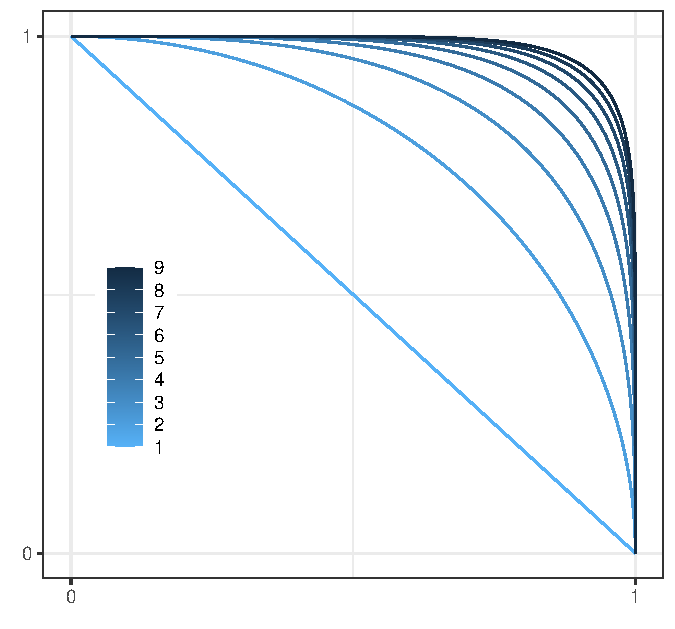
\includegraphics[height=\frametextheight, width = \frametextheight]{./images/p_sphere}
      \end{center}
    \end{column}%
  \end{columns}%
\end{frame} % Unit Sphere - Description
\begin{frame}
  \frametitle{Projection onto the Unit Sphere}
  \begin{itemize}
    \item Take a distribution from $\mathcal{R}_+^{d}$ to $\mathcal{S}_{p}^{d-1}$
    \pause
    \item For finite $p$
      \begin{equation*}
        y_d = \left(1 - {\textstyle\sum}_{l = 1}^{d-1}y_l^p\right)^{\frac{1}{p}}
      \end{equation*}
    \pause
    \item Transformation to Radial, Angular
    \begin{equation*}
        \begin{aligned}
      T(x_1,\ldots,x_d) &= \left(\pnorm{\bm{x}}{p}, \frac{x_1}{\pnorm{\bm{x}}{p}},
                    \ldots , \frac{x_{d-1}}{\pnorm{\bm{x}}{p}}\right) = (r,y_1,\ldots,y_{d-1})\\
                    \pause
    T^{-1}\left(r,y_1,\ldots,y_{d-1}\right) &=
      \left(ry_1,\ldots,ry_{d-1}, r\left(1 - {\textstyle\sum}_{l = 1}^{d-1}y_l^p\right)^{\frac{1}{p}}\right) = (x_1,\ldots,x_d)
      \end{aligned}
    \end{equation*}
    \pause
    Determinant of the Jacobian:
    \begin{equation*}
        \lvert J \rvert = r^{d-1}\left[\left(1 - {\textstyle\sum}_{l = 1}^{d-1}y_l^p\right)^{\frac{1}{p}} +
      {\textstyle\sum}_{l = 1}^{d-1}y_l^p\left(1 - {\textstyle\sum}_{l=1}^{d-1}
          y_l^p\right)^{\frac{1}{p} - 1}\right]
    \end{equation*}
  \end{itemize}
\end{frame} % Unit Sphere - Projection

\subsection{Projected Gamma Family}
\begin{frame}
  \frametitle{Projected Gamma Distribution}
  \begin{itemize}
    \item Assume a product of independent Gammas
      \begin{equation*}
        f(r,\bm{y}) = \prod_{l = 1}^d \text{Ga}\left(ry_l\mid\alpha_l,\beta_l\right)
        \lvert J \rvert I_{\bm{y} \in \mathcal{S}_{p}^{d-1}}
      \end{equation*}
    \pause
    \item Expanded Form
      \begin{equation*}
        f(r,\bm{ y}) = \prod_{l = 1}^{d}
        \left[\frac{\beta_l^{\alpha_l}}{\Gamma(\alpha_l)}(ry_l)^{\alpha_l - 1}
                    \exp\lbrace-\beta_lry_l\rbrace\right]
        \times r^{d-1}\left[y_d - {\textstyle \sum}_{l = 1}^{d-1}y_l^p
                  \left(y_d^p\right)^{\frac{1}{p} - 1}\right]
      \end{equation*}
    \pause
    \item Integrate out radial component; left with distribution on angular
      \begin{equation*}
        \text{PG}(\bm{ y}\mid\bm{ \alpha},\bm{ \beta}) = \prod_{l = 1}^d\left[\frac{\beta_l^{\alpha_l}}{\Gamma(\alpha_l)}y_l^{\alpha_l - 1}\right]
          \times \left[y_d - {\textstyle \sum}_{l = 1}^{d-1}y_l^p\left(y_d^p\right)^{\frac{1}{p} - 1}\right]
          \times \frac{\Gamma({\textstyle\sum}_{l = 1}^d\alpha_l)}{\left({\textstyle\sum}_{l = 1}^d \beta_ly_l\right)^{{\scriptstyle\sum_{l = 1}^d \alpha_l}}}
      \end{equation*}
  \end{itemize}
\end{frame} % Projected Gamma Distribution

\begin{frame}
  \frametitle{Data augmentation}
  \begin{itemize}
    \item Sample from full conditional for $r$
      \begin{equation*}
        r\mid\bm{ \alpha},\bm{ \beta}, y \sim \text{Ga}\left(r\mid{\textstyle\sum}_{l = 1}^d \alpha_l,
              {\textstyle\sum}_{l = 1}^d \beta_ly_l\right).
      \end{equation*}
    \pause
    \item To recover independent Gammas interetation
      \begin{equation*}
        L(\bm{\alpha},\bm{\beta} \mid \bm{r},\bm{y}) \propto
            \prod_{i = 1}^n\prod_{l = 1}^{d}\text{Ga}\left(r_iy_{il}\mid\alpha_l,\beta_l\right)
      \end{equation*}
    \pause
    \item Enabling independent inference between dimensions
      \begin{equation*}
        L(\alpha_l,\beta_l) \propto \prod_{i = 1}^n
                  \text{Ga}\left(r_iy_{il}\mid\alpha_l,\beta_l\right)
      \end{equation*}
  \end{itemize}
\end{frame} % Data Augmentation

\begin{frame}
  \frametitle{Projected Gamma Model}
  \begin{itemize}
    \item Basic Model
        \begin{equation*}
            \begin{aligned}
                \bm{ y}\mid\bm{\alpha},\bm{\beta} &\sim \text{PG}(\bm{ y}\mid\bm{\alpha},\bm{\beta})\\
                \bm{ \alpha},\bm{\beta} &\sim {\textstyle \prod}_{l = 1}^d \text{Ga}(\alpha_l \mid \xi_l,\tau_l)
                    \times {\textstyle \prod}_{l = 2}^d \text{Ga}(\beta_l\mid \zeta_l,\sigma_l).
            \end{aligned}
        \end{equation*}
    \pause
    \item Finite Mixture of Projected Gammas
        \begin{itemize}
            \item embarrassingly parallel
            \item Not presenting results
        \end{itemize}
    \item Dirichlet Process Mixture of Projected (Restricted) Gammas
        \begin{itemize}
            \item Gamma or Log-normal prior / centering distribution
        \end{itemize}
  \end{itemize}
  \vfill
  {\small Note: Projection of Restricted Gammas \emph{(PRG)} sets $\beta_l := 1$ for all $l$.}
\end{frame} % Vanilla Model

\begin{frame}
  \frametitle{Choice of Norm}
  \begin{itemize}
    \item $\bm{V} \in \mathcal{S}_{\infty}^{d-1}$
    \pause
    \item Recall Jacobian of projection from $\mathcal{R}_+^d$ to $\mathcal{S}_{p}^{d-1}$
    \begin{equation*}
        \lvert J \rvert = r^{d-1}\left[\left(1 - {\textstyle\sum}_{l = 1}^{d-1}y_l^p\right)^{\frac{1}{p}} +
        {\textstyle\sum}_{l = 1}^{d-1}y_l^p\left(1 - {\textstyle\sum}_{l=1}^{d-1}
              y_l^p\right)^{\frac{1}{p} - 1}\right]
    \end{equation*}
    \pause
    If $p\to\infty$, then validity dependent upon $y_d = 1$.  If $y_d\neq 1$, then $\lvert J \rvert \to 0^{-1}$.
    \pause
    \item \emph{Difficult} to project density in $\mathcal{R}_+^{d}$ to $\mathcal{S}_{\infty}^{d-1}$
    \pause
    \item Easy to project density in $\mathcal{R}_+^{d}$ to $\mathcal{S}_{p}^{d-1}$ for any finite $p$
    \pause
    \item Project to $\mathcal{S}_{p}^{d-1}$ for large $p$, then project posterior predictive samples
  \end{itemize}
\end{frame}

\section[Model Comparison]{Model Comparison on $\mathcal{S}_{\infty}^{d-1}$}
\subsection{Model Comparison}
\begin{frame}
  \frametitle{Model Comparison on $\mathcal{S}_{\infty}^{d-1}$}
  \begin{itemize}
      \item Density is \emph{difficult}
      \item Multivariate distribution
      \item Have samples from posterior predictive
      \begin{itemize}
            \item Posterior Predictive Loss~\citep{gelfand1998}
                \begin{equation*}
                    D_k^{(i)} = \frac{1}{d}\sum_{l = 1}^{d}\left[\text{Var}(X_{il}) +
                        \frac{k}{k+1}\left(\text{E}[X_{il}] - x_{il}\right)^2\right]
                \end{equation*}
            \item Energy Score~\cite{gneiting2007}
      \end{itemize}
  \end{itemize}
\end{frame}

\begin{frame}
  \frametitle{Energy Score}
  {\scriptsize \citep{gneiting2007}}\\~\vspace{0.2cm}\\
  \begin{itemize}
    \item Generalization of CRPS to multiple dimensions
    \begin{equation*}
      \label{eq:es}
      \text{ES}\left(P,\bm{x}_i\right) =  \text{E}_p g\left(\bm{X}_i, \bm{x}_i\right)
                - \frac{1}{2}\text{E}_p g\left(\bm{X}_i,\bm{X}_i^{\prime}\right)
    \end{equation*}
    \pause
    \item Where $g$ is a negative definite kernel\\
      Euclidean distance is most common
    \pause
    \item What is most appropriate on $\mathcal{S}_{\infty}^{d-1}$?
  \end{itemize}
\end{frame}

\subsection{Distance on $\mathcal{S}_{\infty}^{d-1}$}
\begin{frame}
  \frametitle{$\mathcal{S}_{\infty}^{2}$ - 2 Possible Paths}
  \begin{center}
    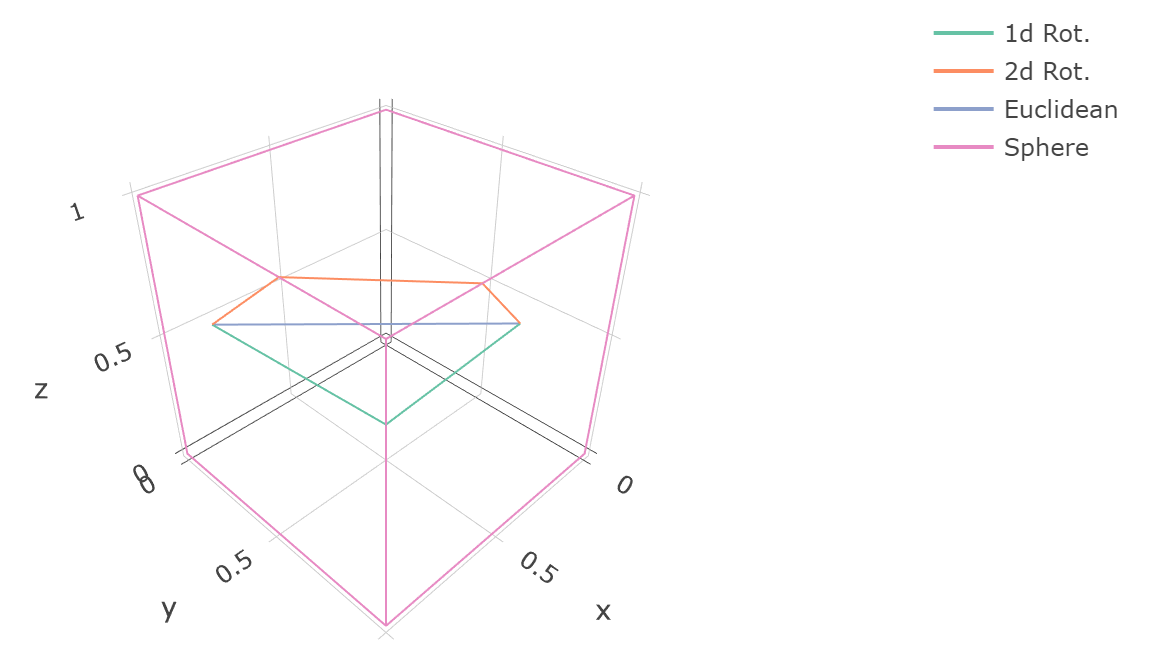
\includegraphics[width=0.8\linewidth]{./images/rotation}
  \end{center}
\end{frame}

\begin{frame}
  \frametitle{Distance on $\mathcal{S}_{\infty}^{d-1}$}
  \begin{itemize}
    \item Length of the shortest path between two points
    \pause
    \item An Unfolded polyhedron is called a \emph{net}
    \pause
    \item If we \emph{Unfold} or \emph{Rotate} $\mathcal{S}_{\infty}^{d-1}$ to the appropriate \emph{net}:
        \begin{itemize}
            \item Shortest distance is length, or \emph{Euclidean distance} of straight line \citep{pappas1989}
            \item \emph{Spider and fly problem}
            \item The \emph{distance} is the length of the shortest line that does not exit the net
        \end{itemize}
  \end{itemize}
\end{frame}

\begin{frame}
    \frametitle{Rotation - 1d and 2d}
    \begin{center}
        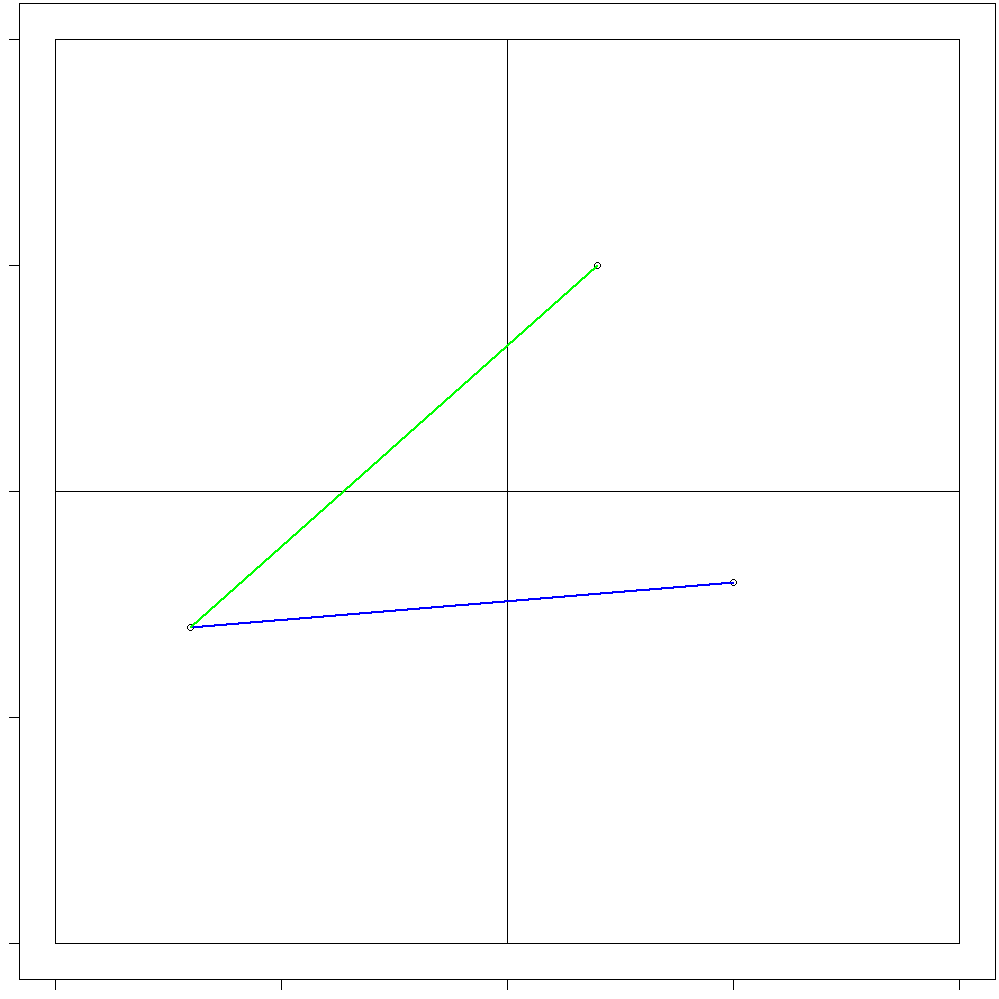
\includegraphics[height = \frametextheight]{./images/rot_3d_2d}
    \end{center}
\end{frame}

\begin{frame}
    \frametitle{Rotation - 3d}
    \begin{center}
        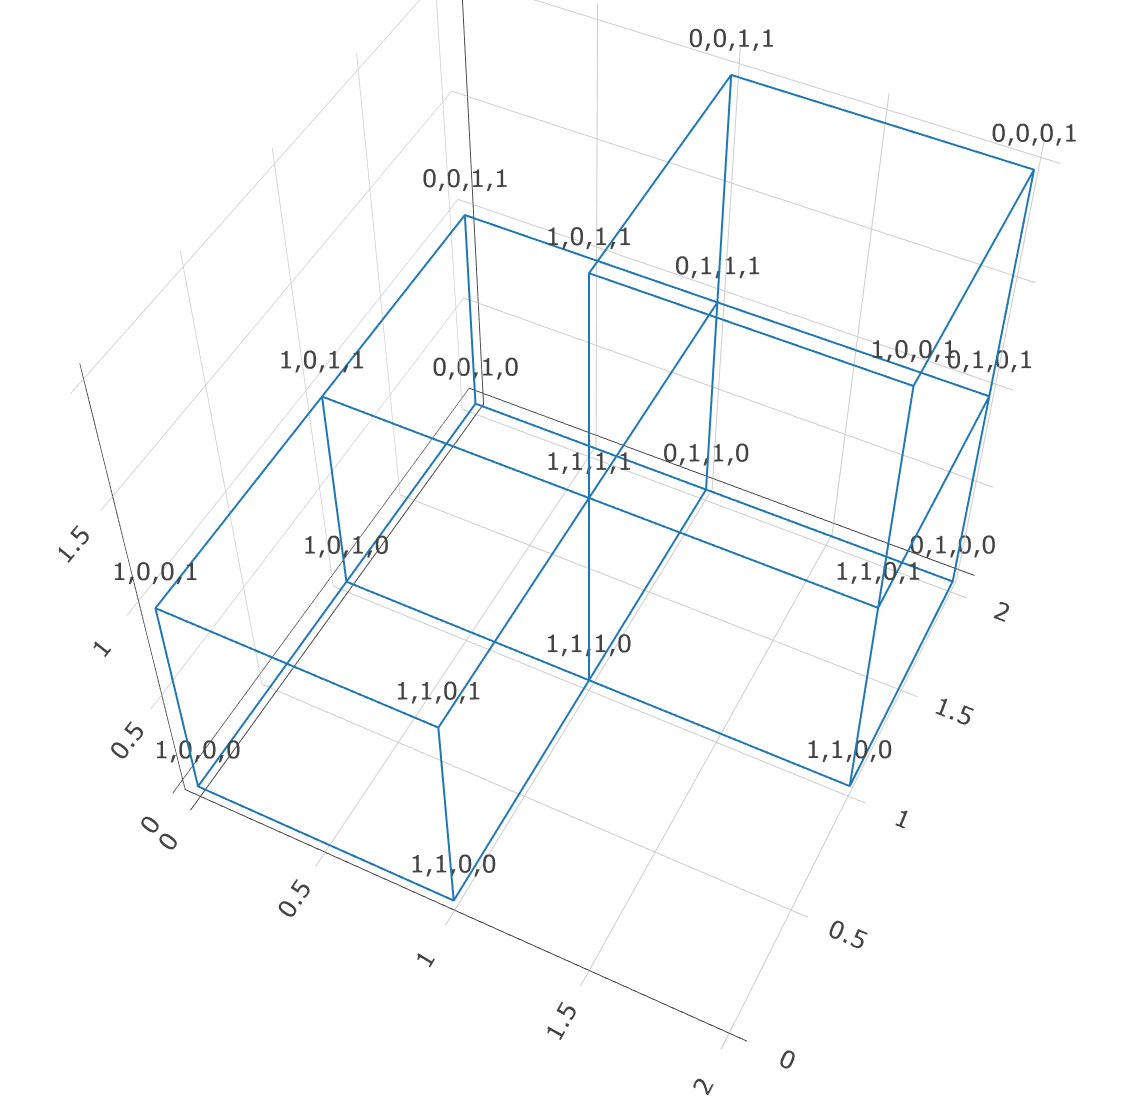
\includegraphics[height=\frametextheight]{./images/rot_4d_3d}
    \end{center}
\end{frame}

\subsection{Negative Definite Kernel on $\mathcal{S}_{\infty}^{d-1}$}
\begin{frame}
  \frametitle{A Valid Negative Definite Kernel}
  \begin{prop}
    For points $a,b \in \mathcal{S}_{\infty}^{d-1}$ a valid negative definite kernel\footnote{A negative definite kernel satisfies symmetry in its arguments, and $\sum_{i = 1}^n\sum_{j = 1}^n \alpha_i\alpha_j g(\bm{x}_1,\bm{x}_2) \leq 0$ for all $x_1,x_2$, for all $\alpha_i$ such that $\sum_{i = 1}^n\alpha_i = 0$.} can be formed as
    \begin{equation*}
      g(\bm{a},\bm{b}) = \begin{cases}
        \pnorm{\bm{b}-\bm{a}}{2} &\text{ if }\argmax_l\bm{a} = \argmax_l\bm{b}\\
        \pnorm{\bm{c}-\bm{a}}{2} + \pnorm{\bm{b}-\bm{c}}{2} &\text{ otherwise}
      \end{cases}
    \end{equation*}
    where $\bm{c}$ resides on intersection between faces of $\bm{a}$ and $\bm{b}$, and
                minimizes $g(\bm{a},\bm{b})$.
  \end{prop}
\end{frame}



\section{Results}

\subsection{Simulation}

\begin{frame}
  \frametitle{Simulation Study}
  \begin{itemize}
    \item Finite mixture of Gammas
    \item For each Number of Mixture Components (3,6,9,12):
      \begin{itemize}
        \item Generate a data-set of 20 columns
        \item output subsets of c = 3,6,12,20 columns projected onto $\mathcal{S}_{\infty}^{c-1}$.
      \end{itemize}
  \end{itemize}
\end{frame}

\begin{frame}
  \frametitle{Simulation - Posterior predictive loss}
  \begin{center}
    \includegraphics[height=\frametextheight]{./images/simulation_ppl}
  \end{center}
\end{frame}

\begin{frame}
  \frametitle{Simulation - Energy Score}
  \begin{center}
    \includegraphics[height=\frametextheight]{./images/simulation_es}
  \end{center}
\end{frame}

\subsection{Integrated Vapor Transport}

\begin{frame}
  \frametitle{IVT - Energy Score}
  \begin{center}
    \include{table_dev}
  \end{center}
\end{frame}

\section[EVT Applications]{Applications of EVT Analysis}
\subsection{EVT Applications}

\begin{frame}
  \frametitle{Applications of EVT Analysis}
  \begin{itemize}
    \item Pairwise Extremal Dependence Coefficients~\citep{warner2018}\\~\vspace{0.3cm}\\
    \item Conditional Survival Functions
  \end{itemize}
\end{frame}

\subsection{Pairwise Extremal Dependence Coefficients}

\begin{frame}
  \frametitle{Pairwise Extremal Dependence Coefficients}
  {\scriptsize\citep{warner2018}}
    \begin{itemize}
      \item A summary measure of extremal dependence
      \begin{equation*}
        \chi_{kl} = \lim\limits_{u\to\infty}\text{P}\left(Z_k > u\mid Z_l > u\right).
      \end{equation*}
      \pause
      \item Bounded to $[0,1]$
        \begin{itemize}
          \item $0$ represents asymptotic independence
          \item A Pareto model can not represent asymptotic independence
        \end{itemize}
      \pause
      \item Reformulated to unit hypercube
        \begin{equation*}
          \chi_{kl} = \text{E}\left[\frac{V_k}{\text{E}(V_k)}{\bigwedge}\frac{V_l}{\text{E}(V_l)}\right]
        \end{equation*}
        Where $\bm{V} = \bm{Z} / \lVert\bm{Z}\rVert_{\infty}$
    \end{itemize}
\end{frame}

\begin{frame}
  \frametitle{IVT - Extremal Dependence}
  \begin{minipage}{.49\textwidth}
    \centering
    \includegraphics[width=0.99\linewidth]{./images/chi_ij_8}
  \end{minipage}
  \begin{minipage}{.49\textwidth}
    \centering
    \includegraphics[width=0.99\linewidth]{./images/chi_ij_46}
  \end{minipage}
\end{frame}

\subsection{Conditional survival functions}

\begin{frame}
  \frametitle{Conditional Survival Function}
  \begin{prop}
      In one dimension, the conditional survival function can be calculated as
   \begin{equation*}
      \label{eqn:condsurv1df}
      \text{P}\left[Z_l > z_l\mid \bm{Z}_{\neg(l)} > \bm{z}_{\neg(l)}\right] =
        \frac{\text{E}\left[\bigwedge_{k = 1}^d \frac{V_k}{z_k}\right]}{
                      \text{E}\left[\bigwedge_{k \neq l}\frac{V_k}{z_k}\right]}
    \end{equation*}
      where $\bm{V} = \bm{Z} / \pnorm{\bm{Z}}{\infty}$.
  \end{prop}
\end{frame}


\begin{frame}
  \frametitle{IVT - Conditional Survival 1d}
  \begin{center}
    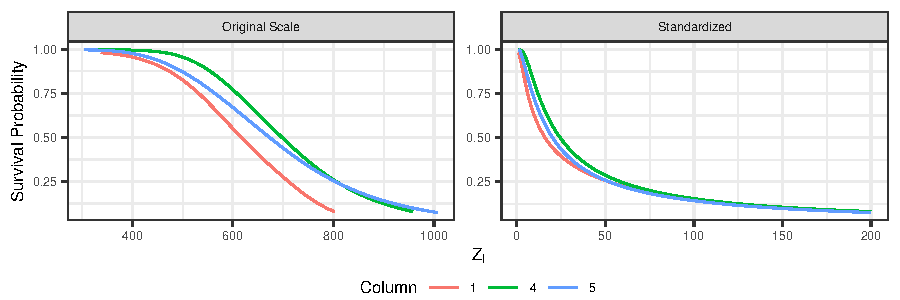
\includegraphics[height=0.8\frametextheight,width=0.9\textwidth]{./images/condsurv_1d}
  \end{center}
\end{frame}

\begin{frame}
  \frametitle{IVT - Conditional Survival 2d (selected)}
  \begin{center}
    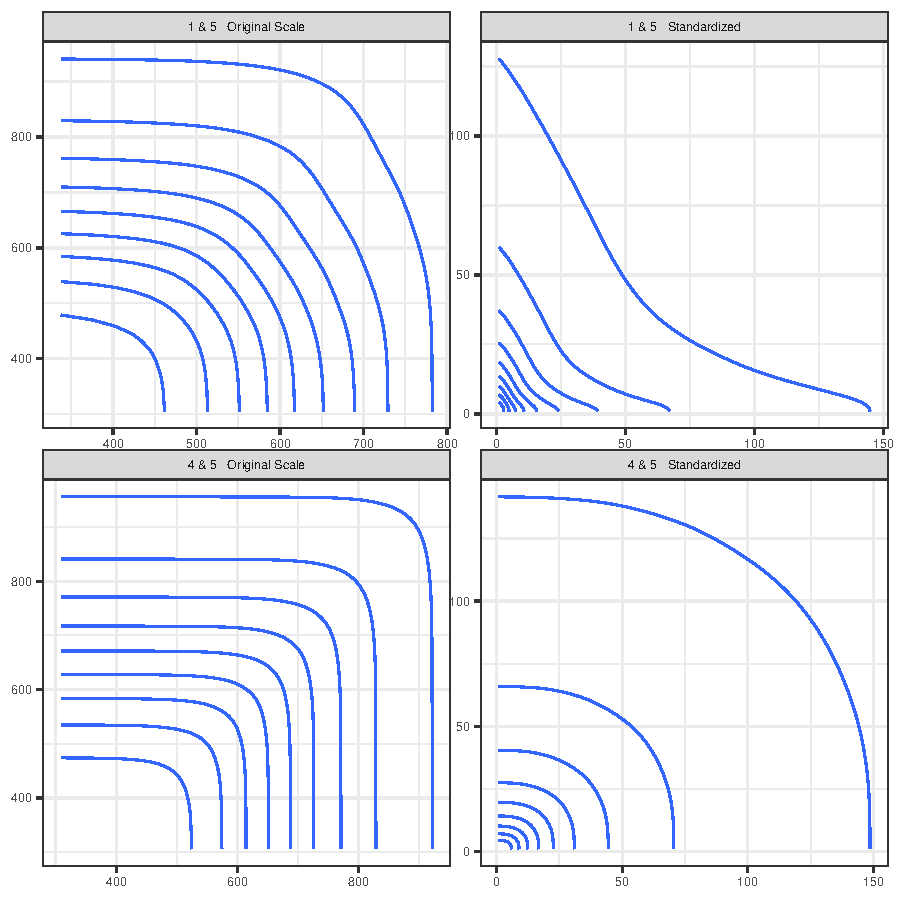
\includegraphics[height=\frametextheight,width=\frametextheight]{./images/condsurv_2d}
  \end{center}
\end{frame}

\section[Anomaly]{Applications to anomaly detection}

\begin{frame}
  \frametitle{What is an anomaly?}
  \begin{itemize}
    \item Anomalies are:
      \begin{itemize}
        \item Observations with large outliers?
        \item Observations with outsized effects?
        \item Data that is \emph{different}.
        \item Data from regions of data sparsity
      \end{itemize}
    \item Desire anomaly \emph{scores}--larger$\rightarrow$more anomalous
  \end{itemize}
\end{frame}

\begin{frame}
  \frametitle{Classical Anomaly Detection Methods}
  \begin{itemize}
    \item Clustering methods
      \begin{itemize}
        \item Linkage-based (single, \dots, complete)~\citep{ackerman2010}
        \item Centroid-based ($k$-Means)~\citep{hartigan1979} 
        \item Density-based (DBSCAN)~\citep{ester1996}
      \end{itemize}
    \item Non-statistical Models
      \begin{itemize}
        \item Isolation Forest~\citep{liu2000}
        \item One-class SVM~\citep{chang2011}
        \item Local Outlier Factor~\citep{breunig2000}
      \end{itemize}
    \item Statistical Models
      \begin{itemize}
        \item Density Estimation routines (GMM's, KDE, KNN)
      \end{itemize}
  \end{itemize}
\end{frame}

\begin{frame}
  \frametitle{Proposed Anomaly Scoring Methods}
  \begin{itemize}
    \item Density Estimation on the hypersphere
    \item Contribution to Posterior Predictive Loss
  \end{itemize}
\end{frame}

\begin{frame}
  \frametitle{Posterior Predictive \emph{Density}}
  \begin{itemize}
    \item Sample from posterior predictive distribution
    \item Density estimate based on \emph{distance} to $k$th nearest neighbor
    \begin{equation*}
        S_{i,(k)}^{-1} =
          \frac{k}{N}\frac{\Gamma\left(\frac{d-1}{2} - 1\right)}{\pi^{\frac{d-1}{2}}D_{k}^{d-1}(V_i)}
    \end{equation*}
    Using the 1d rotation distance estimate established earlier.
  \end{itemize}
\end{frame}

\begin{frame}
    \frametitle{Contribution to Posterior Predictive Loss}
    \begin{equation*}
         S_{i} = \frac{1}{d}\sum_{l = 1}^{d}\left[\text{Var}(X_{il}) +
                        \left(\text{E}[X_{il}] - x_{il}\right)^2\right]
    \end{equation*}
    \begin{itemize}
        \item \emph{Variance} and \emph{Bias} terms
        \item Larger values for both indicate \emph{hard to predict} observation.
        \item Anomalies are \emph{different} from prevailing distribution--PPL would indicate this
    \end{itemize}
\end{frame}

\begin{frame}
  \frametitle{Anomaly Detection Results (Simulated Data)}
  \begin{center}
    \include{table_ad_sim_results}
  \end{center}
\end{frame}

\section[Scaling]{Scaling to higher dimensions}

\begin{frame}
  \frametitle{Scaling to Higher Dimensions}
  \begin{itemize}
    \item Compuitational advances in modelling
      \begin{itemize}
        \item Variational Bayes~\citep{green2015}
      \end{itemize}
    \item Maintaining Model Fidelity at Scale
      \begin{itemize}
        \item Gaussian Mixture prior on $\log\alpha$
        \item $\eta$-Cones~\citep{goix2017}
      \end{itemize}
  \end{itemize}
\end{frame}

\begin{frame}
  \frametitle{Scale - Mixture of Gammas Prior}
  \begin{itemize}
    \item $\eta \subset \lbrace 1,\ldots,d\rbrace$.  Define the $\eta$-Cone:
      \begin{equation*}
        \mathcal{C}_{\eta} = \left\lbrace \bm{z} : z_l > 0 \text{ for }l\in\eta;
                              \hspace{0.2cm} z_l = 0 \text{ for }l\not\in\eta\right\rbrace
      \end{equation*}
    \pause
    \item Gamma models do not have support at 0--$\epsilon$-thickened cones
      \begin{equation*}
        \mathcal{C}_{\eta}^{(\epsilon)} = \left\lbrace \bm{z} : z_l \geq \epsilon
          \text{ for }l\in\eta; \hspace{0.2cm} z_l = 0 \text{ for }l\not\in\eta\right\rbrace
      \end{equation*}
    \pause
    \item How does this help us?
      \begin{itemize}
        \item For Gamma models, $\alpha < 1$ $\implies$ mass near 0
        \item A mixture of gammas for $\alpha_l$:
          \begin{equation*}
            \alpha_l \sim I_{l\in\eta}\text{Ga}(\alpha_l\mid a_1, 1)
                        + I_{l\not\in\eta}\text{Ga}(\alpha_l\mid a_0, 1)
          \end{equation*}
          with $\alpha_0 < 1$, $\alpha_1 > 1$
      \end{itemize}
  \end{itemize}
\end{frame}

\section{Conclusion}

\subsection{Summary}

\begin{frame}
  \frametitle{Conclusion}
  \begin{itemize}
    \item Developed a means of describing the dependence structure of the multivariate Pareto
    \item Demonstrated inherent difficulty in distribution on $\mathcal{S}_{\infty}^{d-1}$
      \begin{itemize}
        \item developed a means of model comparison on the space
      \end{itemize}
    \item Applied models to IVT data
      \begin{itemize}
        \item Pairwise Extremal Dependence Coefficients
        \item Conditional Survival Curves
      \end{itemize}
    \item Anomaly Detection (Preliminary)
    \item Modelling at Scale (on the horizon)
  \end{itemize}
\end{frame}

\subsection{Timeline}

\begin{frame}
    \frametitle{Timeline}
    \begin{center}
        \includegraphics[width=\textwidth]{./images/timeline}
    \end{center}
\end{frame}


\begin{frame}[plain]
    \begin{center}
        
\includegraphics[height=0.7\frametextheight]{./images/fin}
    \end{center}
\end{frame}

\begin{frame}[allowframebreaks]
    \frametitle{References}
    \footnotesize
    \bibliography{./refs}
\end{frame}


\appendix

\section*{Appendix}

\subsection*{IVT}
\begin{frame}
    \frametitle{IVT Grid}
    \begin{minipage}{.49\textwidth}
    \centering
    \includegraphics[height=\frametextheight]{./images/grid_8}
  \end{minipage}
  \begin{minipage}{.49\textwidth}
    \centering
    \includegraphics[height=\frametextheight]{./images/grid_47}
  \end{minipage}
\end{frame}

\subsection*{Projection onto $\mathcal{S}_p^{d-1}$}
\begin{frame}
  \frametitle{Jacobian}
  \begin{equation*}
    \begin{bmatrix}
      y_1 & r & 0 & \ldots & 0\\
      y_2 & 0 & r & \ldots & 0\\
      \vdots & \vdots & \vdots & \ddots & \vdots\\
      y_{d-1} & 0 & \ldots & 0 & r \\
      \left(1 - {\scriptsize\sum_{l=1}^{d-1}}y_l^p\right)^{1/p} &
        - ry_1^{p-1}\phi & -ry_2^{p-1}\phi & \cdots & -ry_{d-1}\phi
    \end{bmatrix}
  \end{equation*}
  where $\phi = \left(1 - {\scriptsize\sum_{l=1}^{d-1}}y_l^p\right)^{1/p - 1}$
  \pause
  \begin{equation*}
  \lvert J \rvert = r^{d-1}\left[\left(1 - {\textstyle\sum}_{l = 1}^{d-1}y_l^p\right)^{\frac{1}{p}} +
      {\textstyle\sum}_{l = 1}^{d-1}y_l^p\left(1 - {\textstyle\sum}_{l=1}^{d-1}
          y_l^p\right)^{\frac{1}{p} - 1}\right]
  \end{equation*}
\end{frame} % Unit Sphere - Jacobian


\subsection*{Projected Gamma Models}

\subsection*{Finite Mixture of Projected Gammas}
\begin{frame}
  \frametitle{Finite Mixture Model}
  \begin{equation*}
    \begin{aligned}
      \bm{ y}_i &\sim \sum_{j = 1}^J\pi_j\text{PG}\left(\bm{ y}\mid \bm{ \alpha}_j, \bm{ \beta}_j\right)\\
      \bm{ \alpha}_j &\sim {\textstyle \prod}_{l = 1}^d \text{Ga}\left(\alpha_l\mid\xi_l,\tau_l\right)\\
      \bm{ \beta}_j &\sim {\textstyle \prod}_{l = 2}^d \text{Ga}\left(\beta_l\mid\zeta_l,\sigma_l\right)
    \end{aligned}
    \hspace{2cm}
    \begin{aligned}
      \bm{ \xi},\bm{\tau} &\sim {\textstyle \prod}_{l = 1}^d \text{Ga}(\xi_l\mid a,b)
                \times \text{Ga}(\tau_l\mid c,d)\\
      \bm{ \zeta},\bm{\sigma} &\sim {\textstyle\prod}_{l = 2}^d\text{Ga}(\zeta_l \mid a,b)
              \times \text{Ga}(\sigma_l\mid c,d)\\
      \bm{ \pi} &\sim \text{Dir}(\pi_0)
    \end{aligned}
  \end{equation*}
\end{frame} % Projected Gamma - Finite Mixture Model

\begin{frame}
  \frametitle{Dirichlet Process Mixture Model}
  \begin{equation*}
    \begin{aligned}
      \bm{ y}_i &\sim \sum_{j = 1}^{\infty}\pi_j\text{PG}\left(\bm{ y}\mid \bm{ \alpha}_j, \bm{ \beta}_j\right)\\
      (\alpha_j,\beta_j) &\sim \text{DP}\left(\eta, G_0\right)\\
      &~\hspace{-1cm}G_0 = {\textstyle\prod}_{l = 1}^d\text{Ga}\left(\alpha_{jl}\mid\xi_{l},\tau_{l}\right)\\
      &~\hspace{0.5cm}\times{\textstyle\prod}_{l=2}^d\text{Ga}\left(\beta_{jl}\mid\zeta_{l}\tau_{l}\right)
    \end{aligned}
    \hspace{1cm}
    \begin{aligned}
      \bm{ \xi},\bm{ \tau} &\sim {\textstyle \prod}_{l = 1}^d \text{Ga}(\xi_l\mid a,b)
              \times \text{Ga}(\tau_l\mid c,d)\\
      \bm{ \zeta},\bm{\sigma} &\sim {\textstyle\prod}_{l = 2}^d\text{Ga}(\zeta_l \mid a,b)
              \times \text{Ga}(\sigma_l\mid c,d)\\
      \bm{ \eta} &\sim \text{Ga}(\eta \mid 2, 0.1).
    \end{aligned}
  \end{equation*}
\end{frame}

\begin{frame}
  \frametitle{Log-normal Prior for Shape Parameters}
  \begin{equation*}
    \begin{aligned}
      \bm{ y}_i &\sim \sum_{j = 1}^{\infty}\pi_j\text{PG}\left(\bm{ y}\mid \bm{ \alpha}_j, \bm{\beta}_j\right)\\
      (\bm{\alpha}_j, \bm{\beta}_j) &\sim \text{DP}\left(\eta, G_0\right)\\
        &~\hspace{-1cm}G_0 = \mathcal{N}\left(\log\bm{ \alpha}_{j}\mid\mu,\Sigma\right)\\
        &~\hspace{0.5cm}\times
            {\textstyle\prod}_{l = 2}^d\text{Ga}\left(\beta_{jl}\mid\zeta_l,\sigma_l\right)
    \end{aligned}
    \hspace{1cm}
    \begin{aligned}
      \mu,\Sigma &\sim \mathcal{N}\left(\mu\mid\mu_0,\Sigma_0\right)
                                  \times \text{IG}\left(\nu,\Psi\right)\\
      \bm{ \zeta},\bm{\sigma} &\sim {\textstyle\prod}_{l = 2}^d\text{Ga}(\zeta_l \mid a,b)
                                \times \text{Ga}(\sigma_l \mid c,d) \\
      \bm{ \eta} &\sim \text{Ga}(\eta \mid 2, 0.1).
    \end{aligned}
  \end{equation*}
\end{frame}

\subsection*{Projected Gamma Inference}
\begin{frame}
  \frametitle{Projected Gamma Model - Inference}
  \begin{itemize}
    \item Full conditional for $\beta_l$
      \begin{equation*}
        \beta_l\mid \bm{ y}, r, \alpha_l \sim \text{Ga}\left(n\alpha_l + \zeta_l,
                {\textstyle \sum}_{i = 1}^nr_iy_{il} + \sigma_l\right)
      \end{equation*}
    \pause
    \item Posterior for $\alpha_l$
      \begin{equation*}
        f(\alpha_l \mid \bm{ y}, r) \propto
          \frac{\left({\textstyle \prod}_{i = 1}^nr_iy_{il}\right)^{\alpha_l - 1}}{
            \Gamma^n(\alpha_l)} \times \alpha_l^{\xi_l - 1}\exp\{-\tau_l\alpha_l\} \times
            \frac{\Gamma(n\alpha_l + \zeta_l)}{
            \left({\textstyle\sum}_{i = 1}^n r_iy_{il} + \sigma_l
                  \right)^{(n * \alpha_l + \zeta_l)}}
      \end{equation*}
    \pause
    \item If $\beta_l = 1$, then
    \begin{equation*}
      f(\alpha_l \mid \bm{ y}, r) \propto
        \frac{\left({\textstyle\prod}_{i = 1}^n r_iy_{il}\right)^{\alpha_l - 1}}{\Gamma^n(\alpha_l)} \times
        \alpha_l^{\xi_1 - 1}\exp\{-\tau_1\alpha_l\}
    \end{equation*}
  \end{itemize}
\end{frame}



\subsection*{Alternative forms of model comparison}
\begin{frame}
  \frametitle{Kullbeck Liebler Divergence}
  \begin{itemize}
    \item KL Divergence
      \begin{equation*}
        D_{\text{KL}}(A,B) = \int_{x\in \Omega(A)}A(x)\log\left(\frac{A(x)}{B(x)}\right)\text{d}x
      \end{equation*}
      requires an estimate of density.
    \pause
    \item We have demonstrated the difficulty of establishing density.  Approximate
      \begin{equation*}
      D_{\text{KL}}^{(k)}(A,B) = \log\frac{n(B)}{n(A)} + c(A) \left[\rho_A^{(k)}(B)
                                                      - \rho_A^{(k)}(A)\right]
      \end{equation*}
  \end{itemize}
\end{frame} % KL Divergence (Introduction)


\subsection*{Alternative Geometries}
\begin{frame}
  \frametitle{Alternative Geometries}
  \small
  \begin{itemize}
    \item Coordinate system to describe $\mathcal{S}_p^{d-1}$ in $\omega^{d-1}$
    \item $\mathcal{L}_1$: Log-ratios \citep{aitchison1982}:
        \begin{equation*}
            \mathcal{S}_1^{d-1} \rightarrow (-\infty,\infty)^{d-1}\hspace{8cm}~
        \end{equation*}
    \item $\mathcal{L}_2$: Spherical Coordinates \citep{nunez2019}: 
        \begin{equation*}
            \mathcal{S}_2^{d-1} \rightarrow [0,\pi/2]^{d-1}\hspace{8cm}~
        \end{equation*}
        \vspace{-0.5cm}
      \begin{equation*}
        \begin{aligned}
        \theta_l &= \cos^{-1}\left(\frac{y_l}{\lVert \bm{y}_{l:d}\rVert_2}\right)\\
        &\hspace{0.75cm}\text{for }l = 1,\ldots,d-1
        \end{aligned}
        \hspace{1cm}
        \begin{aligned}
          y_1 &= \cos\theta_1\\
          y_l &= \left[{\textstyle\prod}_{k = 1}^{l-1}\sin\theta_k\right]\cos\theta_l\\
          &\hspace{0.75cm}\text{for }l = 2,\ldots,d-1\\
          y_d &= {\textstyle\prod}_{k = 1}^{d-1}\sin\theta_k
        \end{aligned}
      \end{equation*}
  \end{itemize}
\end{frame}
\begin{frame}
  \frametitle{Probit-Normal}
  Let $Q_i = \text{Probit}(2\theta_i / \pi)$, for $i = 1,\ldots,d-1$
  \begin{equation*}
    \begin{aligned}
                Q_i &\sim \mathcal{N}_{d-1}\left(\bm{\mu}_i, \Sigma_i\right)\\
    \bm{\mu}_i, \Sigma_i &\sim \text{DP}(\eta, G_0)\\
                    &\hspace{-1cm}G_0 =
                      \mathcal{N}_{d-1}(\bm{\mu}_i\mid\bm{\mu}_0,\Sigma_0)\times \text{IW}(\Sigma_i\mid\nu,\Psi)
    \end{aligned}
    \hspace{1cm}
    \begin{aligned}
              \mu_0 &\sim \mathcal{N}_{d-1}\left(\bm{u},\bm{S}\right)\\
           \Sigma_0 &\sim \text{IW}(\nu_0,\Psi_0)\\
               \eta &\sim \text{Ga}(\alpha, \beta)
    \end{aligned}
  \end{equation*}
\end{frame}

\subsection*{Negative Definite Kernel}
\begin{frame}
    \frametitle{Negative Definite Kernel - Proof}
    \begin{itemize}
        \item In the first case, where $\bm{a}$ and $\bm{b}$ $\rightarrow$ Euclidean distance. 
        \item In the second case, $\bm{a}$ and $\bm{b}$ reside on separate
  faces.  
  \begin{itemize}
      \item $c$ is unique, $\pnorm{\bm{c} - \bm{a}}{2} = \pnorm{\bm{a} - \bm{c}}{2}$ $\rightarrow$ symmetry in the arguments.
      \item Then for the other property of negative definiteness
  \begin{equation*}
    \begin{aligned}
      \sum_{i = 1}^n\sum_{j = 1}^n \alpha_i\alpha_j g(\bm{x}_1,\bm{x}_2) &= \sum_{i = 1}^n\sum_{j = 1}^n \alpha_i\alpha_j \bigg[\pnorm{\bm{c} - \bm{x}_1}{2} + \pnorm{\bm{x}_2 - \bm{c}}{2}\bigg]\\
      &= \sum_{i = 1}^n\sum_{j = 1}^n \alpha_i\alpha_j\pnorm{\bm{c} - \bm{x}_1}{2} + \sum_{i = 1}^n\sum_{j = 1}^n \alpha_i\alpha_j\pnorm{\bm{x}_2 - \bm{c}}{2}
    \end{aligned}
  \end{equation*}
  which is less than or equal to $0$ in both terms
  \end{itemize} 
  \end{itemize}
\end{frame}

\subsection*{Simulation - Alternative Model Selection Criteria}


\begin{frame}
  \frametitle{Simulation - KL Divergence}
  \begin{center}
    \includegraphics[height=\frametextheight]{./images/simulation_knn_kld}
  \end{center}
\end{frame}

\subsection*{IVT - Alternative Selection Criteria}

\begin{frame}
  \frametitle{IVT - KL Divergence}
  \begin{center}
    \includegraphics[height=\frametextheight]{./images/knn_kld}
  \end{center}
\end{frame}

\subsection*{Conditional Survival}

\begin{frame}
  \frametitle{Conditional Survival Function - Proof}
  {\small
  \begin{equation*}
    \label{eqn:condsurv1d}
    \text{P}\left[Z_l > z_l\mid \bm{Z}_{-(l)} > \bm{z}_{-(l)}\right] =
      \frac{\text{P}\left[\cap_{k = 1}^d Z_k > z_k\right]}{\text{P}\left[\cap_{k \neq l} Z_k > z_k\right]}.
  \end{equation*}
  \pause
  $R = \pnorm{\bm{Z}}{\infty}$, $\bm{V} = \frac{\bm{Z}}{R}$, such that
    $\bm{V}\in \mathcal{S}_{\infty}^{d-1}$.  Then $\bm{Z} = R\bm{V}$.
  \begin{equation*}
    \text{P}\left(\cap_{k = 1}^d Z_k > z_k\right) = \text{P}\left(\cap_{k = 1}^d RV_k > z_k\right)
  \end{equation*}
  \pause
  Recall, for standard Pareto, $\text{P}(R > r) = 1\wedge\frac{1}{r}$.
  \begin{equation*}
    \text{P}\left[\bigcap_{k = 1}^d R > \frac{z_k}{v_k}\right] =
      \text{P}\left[R  > \bigvee_{k=1}^d\frac{z_k}{V_k}\right] =
      \text{E}\left[1 \bigwedge \left(\bigvee_{k = 1}^d\frac{z_k}{V_k}\right)^{-1}\right]
  \end{equation*}
  $V_k \in [0,1]$; $z_k > 1$ (for the region of interest) $\implies$ $\frac{z_k}{V_k} > 1$
  }
\end{frame}

\begin{frame}
    \frametitle{Conditional Survival Function - Proof Cont.}
    {\small 
  \begin{equation*}
    \text{P}\left[\cap_{k = 1}^d Z_k > z_k\right] = \text{E}\left[\wedge_{k = 1}^d\frac{V_i}{z_i}\right].
  \end{equation*}
  \pause
  And similar for the denominator
  \begin{equation*}
    \text{P}\left[Z_l > z_l\mid \bm{Z}_{\neg(l)} > \bm{z}_{\neg(l)}\right] =
      \frac{\text{E}\left[\wedge_{k = 1}^d \frac{V_k}{z_k}\right]}{\text{E}\left[
                \bigwedge_{k \neq l}\frac{V_k}{z_k}\right]}
  \end{equation*}
  }
\end{frame}



\end{document}
